\documentclass{article}
\usepackage{a4}
\usepackage{fullpage}
\usepackage{url}
\usepackage{graphicx}
\parindent 0pt
\parskip 6pt
\begin{document}
\large
\begin{center}
{\bf Providing mains power to masts}
\end{center}

Connecting a mast to the mains  is straightforward, but some care is
needed if the mast is some distance -- maybe 1000m -- from the power
source.  First, you will be using armoured cable which, at the time of
writing, can be bought for  under \pounds1 per metre. Armoured
cable requires special underground junctions -- be sure to use the
epoxy kind --  and terminals (called
glands), but these are all straightforward to use.  Cable should also
be buried. The method and depth depends on the land and the
wishes of the landowner. I have had quote of \pounds1 per metre for
burying cable over quite rugged ground, so even when properly dug in,
cable may be a cheaper alternative to solar and wind power for all but
the most remote masts.

Cable weighs 300-400kg per 1000m and comes in big drums.  If you have
some sort of buggy like an Argocat that can reach the mast, you may be
able to rig up an axle to support the drum and unroll it as you drive
up the hill.  Alternatively you can cut it into sections of 200-300m
and have some kind of Egyptians and Israelites event when you drag it
up the hillside.  In fact the cable is quite slithery and dragging it
over grass and heather is surprisingly easy.

[There's more to say about power consumption so the following
  paragraph should be expanded and go elsewhere as it applies to
  solar/wind powered masts as well]

Wireless equipment consumes relatively little power. For example, the
manufacturers blurb on the Ubquiti
Rocket\footnote{\url{http://www.ubnt.com/downloads/datasheets/rocketm/rm_ds_web.pdf}}
says 6.5W which agrees well with what I have measured (I measured the
power at the mains -- including the adapter -- and under heavy
traffic, which can increase the power draw).  So a typical mast installation
consisting of two long distance links and one or two wireless cards
for local distribution is probably going to be around 30W (remember to add in the
power required by an ethernet switch).

To keep the cost  to a minimum, you will want to use the smallest
diameter copper core, 1.5mm$^2$.  The resistance of this is given as
about 12 ohms per 1000m.  Given that we know the power required by the
equipment and the cable length we can calculate the the
voltage drop on the line.\footnote{
Let
$V_E$ = voltage across equipment,
$V_D$ = voltage drop on cable,
$V_S$ = voltage at source ($V_S = V_D + V_E$),
$R_C$ = resistance of cable, and
$W_E$ = power required by equipment.
If $I$ is the current through the cable, we have $V_EI  = W_E$, $V_D/R_C
= I$ so $V_EV_D = W_ER_C$  so that $V_E^2 - V_SV_E + W_ER_C = 0$.
From high-school math, $V_E = 1/2(V_S \pm \sqrt{V_S^2 -4W_ER_C})$ or
$V_E = 1/2(V_S \pm \sqrt{V_S^2 -8W_ERL})$ where $L$ is the length of
the cable and $R$ the resistance per unit length of the conductor --
remember there are two conductors!}
The following table assumes a source voltage of 230V and shows the
voltage at the mast for varying cable lengths $L$ and power
consumptions $W_E$.

{\small
\input{droptable1.tex}
}

Most power adapters work over a wide range of voltages, so you can
power a substantial amount of wireless kit without difficulty.  But
once you have mains power at a mast it is tempting to use it for other
things like power tools.  Be careful!  It won't damage a long cable, which
will just get slightly warm, but it may not be good for your tools.

{\bf Safety considerations}

Once you have installed the cable, use a meter to check that
there is no leakage to earth from either conductor.  Also check the
total resistance of the conductors (connect the two at one end and
measure the resistance at the other -- being sure that the whole thing
is unplugged when you do this!)  If you are using 1.5mm$^2$ cable, you
should see something that is about $12\Omega$ per kilometre.  For
example a 1.5km cable should give about $36\Omega$ (remember you are
measuring the sum of the resistances of the two conductors).

Whatever the rules about digging in cable, I believe that by far the
best safety measure is a {\em residual
current device} (RCD). They are standard for garden equipment and
required in some countries for outdoor wiring and wiring in kitchens
and bathrooms.
What these gizmos do is to detect the
difference in the current flowing up the cable and that flowing back.
If there is a difference it is probably the result of a leak to earth
caused by a cable fault or an inquisitive hiker putting his fingers in
your kit. If this happens, the power is disconnected immediately.
Try to get a {\em latching} RCD.  These come back on after a
power cut.

Now we have experienced problems with RCDs on long cables: they trip
for no obvious reason.  I suspect, though I have not done the sums,
that this can be caused by spikes on the power supply.  The theory is
that 
capacitance of the cable is such that a spike {\em on the power supply} on one conductor will be
absorbed in the cable causing a temporary difference.  I need to check
this with a power engineer, but we have found that adding an isolating transformer solves
the problem.  Try to get one that provides the power you
want\footnote{See, for example, \url{http://uk.rs-online.com/web/p/products/0504167}}, the big
ones that are designed for  heavy-duty equipment outdoors waste a lot of
electricity. This picture shows the wiring.  The indicator light is a
good idea: it provides an easy check that the power supply is working.
\begin{figure}
\begin{center}
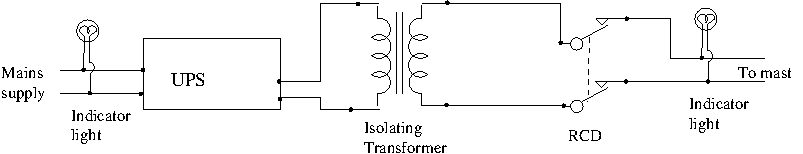
\includegraphics[scale=0.7]{isolating}
\end{center}
\caption{Wiring diagram for power supply at base}
\end{figure}

\begin{figure}
\centerline{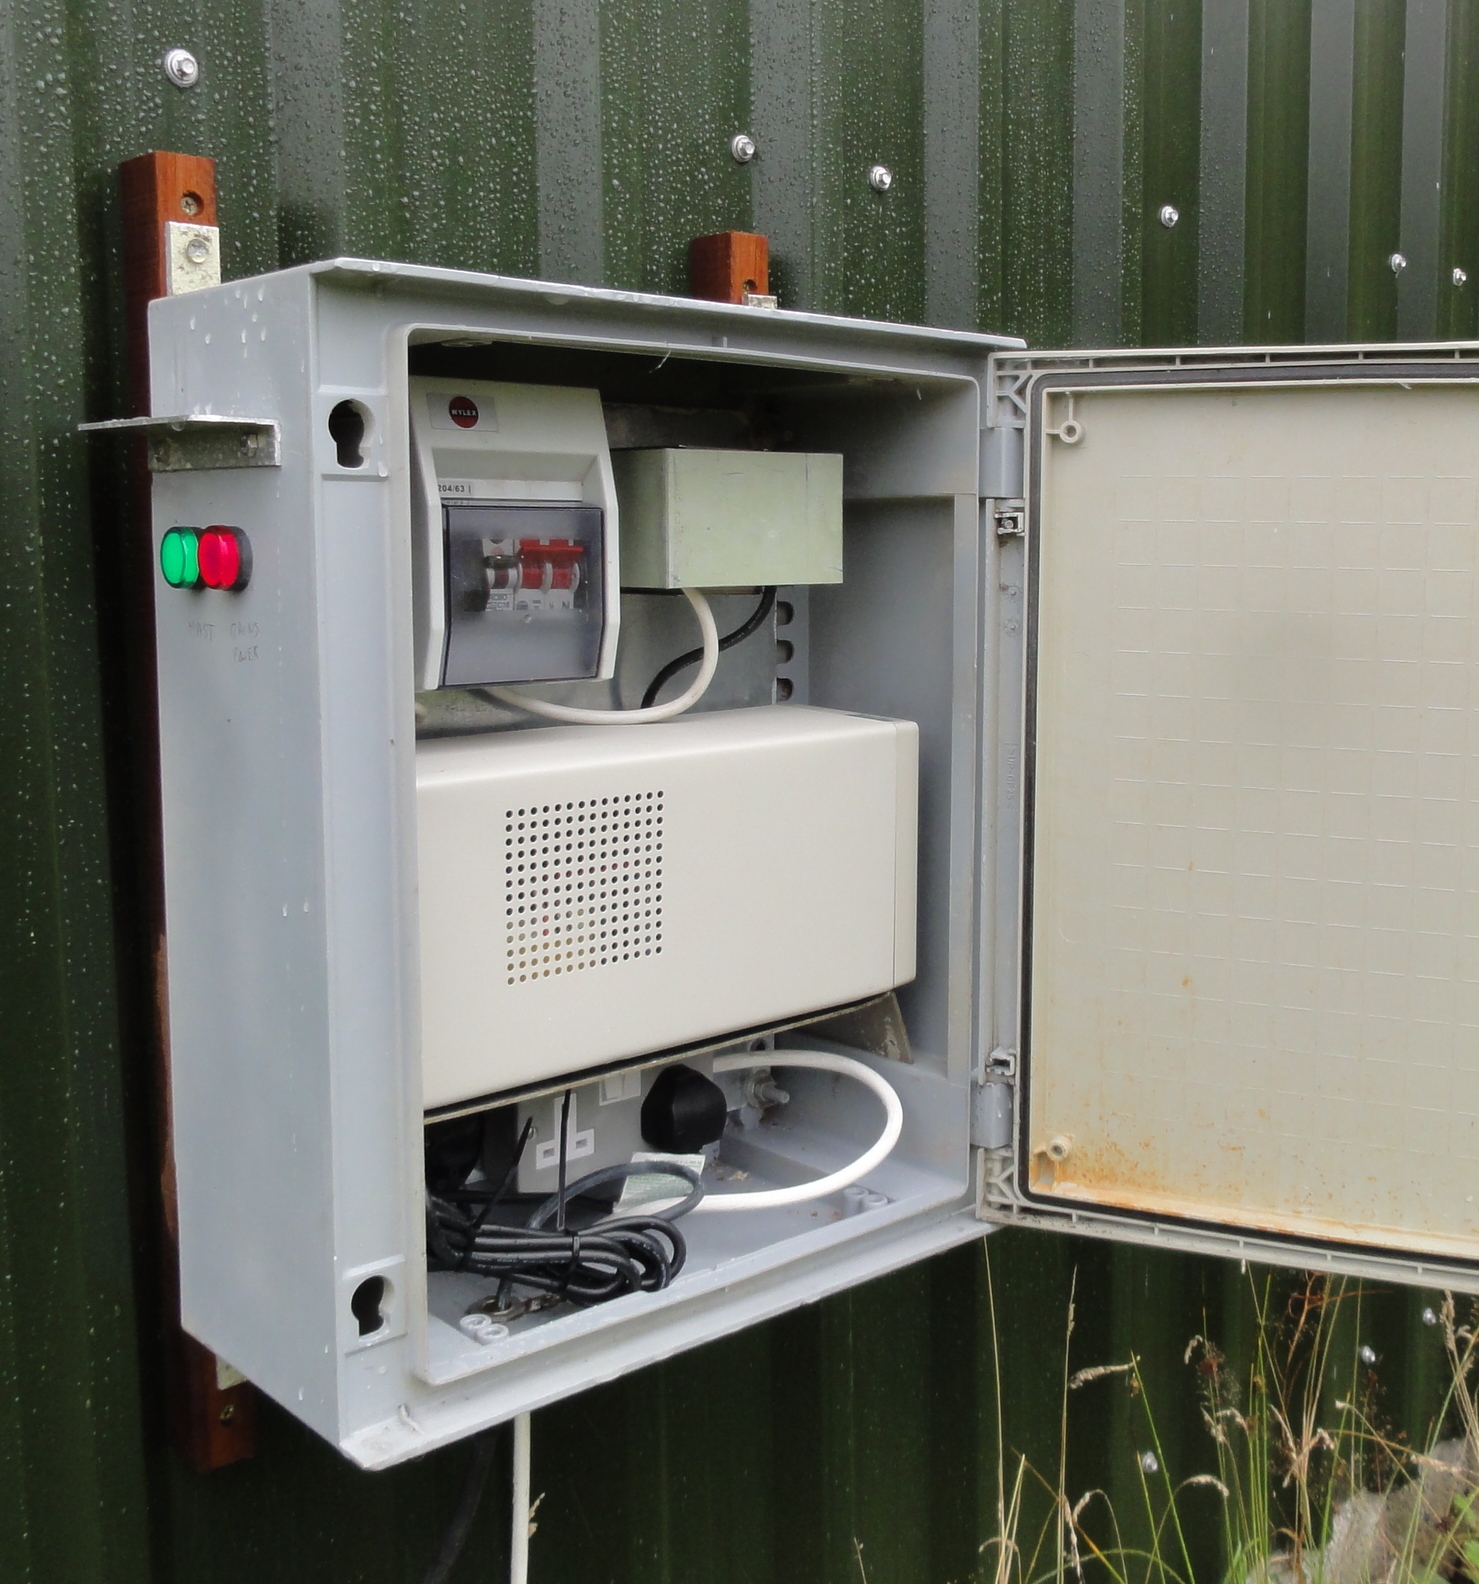
\includegraphics[scale = 0.15,bb= 200 0 1000 1200]{powerbox.jpg}}
\caption{Power supply box showing RCD (top left), isolating
  transformer (top right, behind cover) and UPS (bottom)}
\end{figure}
{\bf Backup}

Rural electricity supplies are unreliable, so you may also want to put
a backup power supply (UPS) at the source.  About \pounds200 buys
you\footnote{\url{http://www.apc.com/products/family/index.cfm?id=27}}
a supply which is quoted as providing 38 minutes at 200W.  For 30W you would
presumably get about about 6 times that -- over 4 hours.  

If you, want to provide backup that lasts for days rather than hours,
you can buy a humongous UPS, but these are very expensive, and an
alternative is to build one yourself with equipment designed for
caravans.  Caravaners have less money than IT departments, so the
savings can be substantial\footnote{Roughly, you get a large car/truck battery.  A 12V 125AH battery
should last 2 days with a 30W draw, and you can connect two or more in
parallel if you want a longer period.  You also need an inverter and a
relatively beefy charger that is designed to be used continuously.  I
haven't done this yet, so I don't want to give more details.  Such
a system would obviate the need for an isolating transformer,
but it may waste electricity to have the inverter running
all the time. In which case you would add a relay to switch to battery
only when the mains supply fails (this is what a UPS does); and you will then need an isolating
transformer.}.

\hfill\begin{tabular}{l}Peter Buneman\\Draft of 15 October 2011
\end{tabular}
\end{document}

===============================

Hi Al,

The resistance of 1400m of 1.5mm2 cable is  about 34 ohms.  If you
draw 30W, the voltage drop from 240V is about 4.5V.  Even if you were
drawing 100W, the drop would be 15V.  The power adapters all work in
the range 120-240V so you are safe.

I tested the power needed for a Rocket (including the ad apter).  It's
about 5W (it may rise a bit with traffic).  I don't know what the
powerbridges draw, but I imagine it's the same, so I think your
estimate is good.  Be sure to check the resistance of the cable once
you have installed it.

We wanted to put an RCD on the bottom of a 1200m cable up the side of
Beinn Sgritheall in order to protect people who might mess with the
cable or the kit, but it kept tripping.  I believe it was spikes on
the supply that were causing this.  We put in an isolating transformer
and now everything is fine.

Finally, why put the UPS at the mast?  I suppose if the cable fails,
the mast will keep running for another day, but how will you know that
the cable has failed?nh

Best wishes

Peter
